% K_static sweep -- Delta vs static-K with peak at K=6
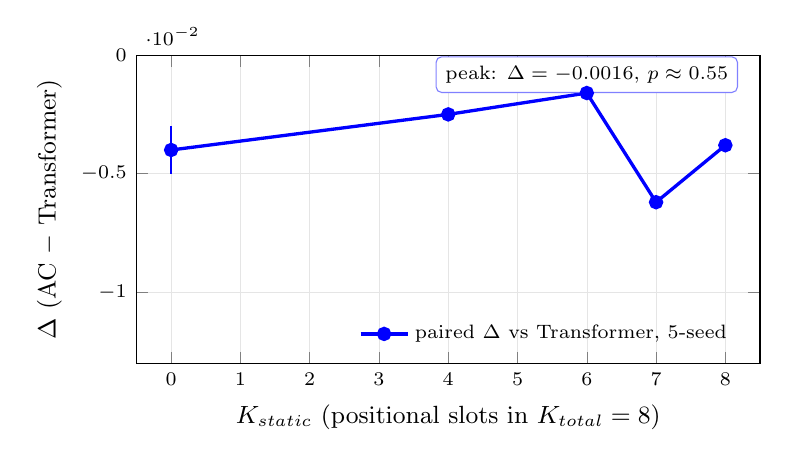
\begin{tikzpicture}
\begin{axis}[
  width=9.5cm, height=5.5cm,
  xlabel={$K_{\text{static}}$ (positional slots in $K_{\text{total}} = 8$)},
  ylabel={$\Delta$ (AC $-$ Transformer)},
  xlabel style={font=\small},
  ylabel style={font=\small},
  tick label style={font=\scriptsize},
  xmin=-0.5, xmax=8.5,
  ymin=-0.013, ymax=0,
  xtick={0,1,2,3,4,5,6,7,8},
  grid=both,
  major grid style={lightgray!40, very thin},
  minor grid style={lightgray!20, very thin},
  legend pos=south east,
  legend style={font=\scriptsize, draw=none, fill=none},
]
% Measured points
\addplot[blue, very thick, mark=*, mark size=2pt] coordinates {
  (0, -0.0040)
  (4, -0.0025)
  (6, -0.0016)
  (7, -0.0062)
  (8, -0.0038)
};
\addlegendentry{paired $\Delta$ vs Transformer, 5-seed}

% Error bars manually approximate
\draw[blue, thick] (axis cs:0, -0.0040) -- (axis cs:0, -0.0040+0.0010);
\draw[blue, thick] (axis cs:0, -0.0040) -- (axis cs:0, -0.0040-0.0010);

% Annotate peak
\node[anchor=south, font=\scriptsize, fill=white, draw=blue!50, rounded corners=2pt]
  at (axis cs:6, -0.0016) {peak: $\Delta = -0.0016$, $p \approx 0.55$};

\end{axis}
\end{tikzpicture}
